\documentclass[10pt,conference]{IEEEtran}

\usepackage{cite}
\usepackage{amsmath,amssymb,amsfonts,amsthm}
\usepackage{booktabs}
\usepackage{array}
\usepackage{multirow}
\usepackage{graphicx}
\usepackage{url}
\usepackage{xcolor}
\usepackage[colorlinks=true, linkcolor=black, citecolor=black, urlcolor=blue]{hyperref}
\usepackage{algorithm}
\usepackage{algorithmic}
\usepackage{tikz}
\usetikzlibrary{arrows.meta,positioning,fit,calc}

\setlength{\textfloatsep}{4pt plus 1pt minus 2pt}
\setlength{\floatsep}{4pt plus 1pt minus 2pt}
\setlength{\intextsep}{4pt plus 1pt minus 2pt}
\setlength{\abovecaptionskip}{2pt}
\setlength{\belowcaptionskip}{0pt}
\renewcommand{\arraystretch}{0.96}

\newtheorem{definition}{Definition}
\newtheorem{theorem}{Theorem}
\newtheorem{proposition}{Proposition}
\newtheorem{corollary}{Corollary}
\newtheorem{remark}{Remark}

\DeclareMathOperator{\Var}{Var}
\newcommand{\E}{\mathbb{E}}
\newcommand{\method}{\textnormal{\mbox{RAMS}}}
\newcommand{\tpatchinst}{\textnormal{\mbox{RAMS-tPatch}}}
\newcommand{\kafinst}{\textnormal{\mbox{RAMS-KAFNet}}}
\newcommand{\baseT}{\textnormal{\mbox{tPatchGNN}}}
\newcommand{\baseK}{\textnormal{\mbox{KAFNet}}}

\begin{document}

\title{RAMS: Mechanism-State Residual Operators for Wearable IMTS Forecasting}

\author{\IEEEauthorblockN{Yangyang Li, Yupeng Sun, Lei Zhang}
\IEEEauthorblockA{Capital Normal University}}

\maketitle

\begin{abstract}
Wearable IMTS forecasting is difficult because sensor reliability, coverage,
and group-asynchronous observation patterns are predictive mechanisms, not
incidental missingness.  Strong IMTS backbones learn value-level states, but
value-similar wearable windows can retain different post-backbone residuals
when their mechanism states differ.  We propose \method{}, a
backbone-agnostic mechanism-state residual operator.  Given a trained
forecaster \(F_0\), \method{} freezes \(F_0\), builds a deployment-valid
mechanism state \(M=(V,R)\), and adds a closed-gated local/integral residual
that is zero at initialization.  We formalize mechanism-state aliasing as a
residual frontier and instantiate the same operator on \baseT{} and \baseK{}.
\tpatchinst{} achieves the best same-protocol reproduced MSE/MAE among public
IMTS backbones on MHEALTH, OPPORTUNITY, and PAMAP2, and stays positive under an
8-epoch strong-backbone check.  \kafinst{} improves matched frozen \baseK{}
checkpoints on HumanActivity and the three wearable-suite datasets, winning all
12 paired dataset--seed comparisons on both MSE and MAE.  These results show
that mechanism-state residuals are a transferable route to more accurate
group-asynchronous wearable forecasting.
Code is available at this repository: \url{https://github.com/anonymousUser-dot/RAMS}.
\end{abstract}

\begin{IEEEkeywords}
Irregular time series, wearable sensing, human activity, forecasting,
temporal patch graphs, residual learning.
\end{IEEEkeywords}

\section{Introduction}

Irregular multivariate time series (IMTS) are common in mobile health and
activity sensing.  Due to sensor contact, power management, body placement, and
activity-dependent motion, wearable streams often contain asynchronous
observations from multiple sensor groups.  The goal is not to reconstruct a
complete signal for its own sake, but to predict future multivariate sensor
values accurately from the observed history.

For this task, a natural strategy is to learn a strong value-level backbone
over all observed values.  Recent backbones include temporal patch graphs,
kernel-aligned forecasters, attention models, and graph models.  They are
competitive because they summarize irregular histories into predictive latent
states.  However, such states can still be value-level summaries.  When two
wearable windows have similar observed values but different coverage, recency,
or group reliability, the backbone may map them to similar states even though
their forecast residuals differ.

Another natural strategy is to add a generic adapter or residual head after a
strong backbone.  This can increase capacity, but it does not explain which
post-backbone information is allowed to improve prediction.  In wearable IMTS,
the useful residual information must be available at deployment and tied to the
sensing mechanism: recent reliability, effective counts, time span, coverage
integrals, and observed value moments.  A generic residual head can therefore
learn spurious corrections, while a value-only backbone can miss
mechanism-dependent corrections.

Figure~\ref{fig:architecture} gives the roadmap of our solution.  Step 1 starts
from any trained IMTS backbone \(F_0\), rather than replacing it.  Step 2
extracts deployment-visible mechanism state \(M=(V,R)\), where \(V\) represents
observed value moments and integrals and \(R\) represents reliability and
coverage.  Step 3 constructs local and integral residual features for each
forecasted time--channel entry.  Step 4 uses a closed-initialized gate to admit
a small correction to the backbone forecast.  This design is intentionally
level-preserving: before residual training, the model is exactly \(F_0\).

We call the underlying failure mode \emph{mechanism-state aliasing}.  Let
\(F_0\) be the backbone, \(Z=Y-F_0(X)\) its residual, \(L\) the value-level
state, and \(M\) the mechanism state.  If
\(\E[Z\mid L,M]\neq\E[Z\mid L]\), then a value-only backbone leaves a residual
frontier even when its value dynamics are strong.  The squared-loss size of the
frontier is
\begin{equation}
\mathcal{F}_M(F_0)=
\E\|\E[Z\mid L,M]-\E[Z\mid L]\|^2 .
\end{equation}
This identity directly motivates our method: preserve \(F_0\), expose \(M\) to
the residual, and keep the residual class small enough that it targets the
frontier rather than relearning the backbone.

The main contributions are summarized as follows:
\begin{itemize}
\item We define the targeted problem of improving strong frozen-backbone
forecasting on group-asynchronous wearable IMTS, and we state the observable
conditions used by the model.
\item We derive a mechanism-state aliasing theory: the exact squared-loss gap
between value-only and mechanism-state residual prediction is
\(\mathcal{F}_M(F_0)\), and a wearable source condition explains when this
frontier is positive.
\item We propose \method{}, a level-preserving residual operator that can be
attached to a frozen IMTS backbone through protocol-valid mechanism summaries,
local/integral branches, and a closed-initialized learned gate.
\item We instantiate the same operator on two backbones: \tpatchinst{} for a
temporal patch graph and \kafinst{} for a kernel-aligned forecaster.  We report
shared-protocol public baselines, paired 4-epoch and 8-epoch \baseT{} results,
four-dataset \baseK{} paired results, mechanism-state controls, and
theorem-aligned diagnostics.
\end{itemize}

\section{Related Work}

\textbf{Irregular time-series forecasting.}
Classical IMTS models handle missingness and irregular sampling with recurrent
decay, continuous-time latent dynamics, set functions, and attention over
observed events \cite{grud,brits,latentode,seft,mtan}.  They are broad, but do
not separate nuisance missingness from informative wearable sensing.  We follow
the missing-data view that an observation mechanism can be informative
\cite{rubin}, and specialize it to wearable forecasting.

\textbf{Graph and patch models.}
Graph and patch IMTS models, including GraFITi and \baseT{}
\cite{grafiti,tpatchgnn}, represent irregular observations as graph or patch
structures.  Our baseline scan confirms that \baseT{} is the strongest
reproduced public IMTS backbone under the shared protocol on the main wearable
suite.  \method{} treats it as one frozen value-dynamics backbone and adds a
mechanism-state residual operator.

\textbf{Missing-value MTS prediction in BigData.}
LIFE \cite{life} shows that missing-value MTS prediction can benefit from
learning features matched to the missingness structure, while joint local/global
models \cite{jointlocalglobal} emphasize that different temporal scales can
matter under missing observations.  \method{} addresses a different failure
mode: after a strong IMTS backbone has already modeled value dynamics,
wearable mechanism states can still split the post-backbone residual inside
value-matched windows.

\textbf{Modern forecasting backbones.}
General time-series forecasting has advanced through transformer variants,
decomposition models, patching, and graph learning
\cite{informer,autoformer,timesnet,patchtst,mtgnn}.  Recent IMTS work revisits
canonical pre-alignment through \baseK{} \cite{kafnet}, while \baseT{} avoids
sequence explosion by transformable patching and time-adaptive graphs.
\method{} is complementary to both: it keeps the chosen backbone fixed and
models a deployment-visible mechanism residual that the backbone leaves behind.

\textbf{Wearable sensing and activity streams.}
Wearable human-activity sensing has long been studied as a multi-sensor,
body-location-dependent recognition problem \cite{lara}.  The forecasting
setting studied here differs from classification, but it inherits the same
physical structure: sensor placement, body contact, and activity phase affect
which channels are reliable.  In activity streams, the same future horizon may
be easier or harder depending on whether multiple body-location groups were
recently reliable.  This motivates treating the wearable observation state as a
predictive object rather than as only missing-value nuisance.

\textbf{Residual forecasting.}
Adapters and residual heads can correct a trained predictor.  Here the residual
is tied to a measurable post-backbone error source: mechanism-state aliasing
inside value-matched wearable windows.  The evaluated target is lower MSE/MAE
on a public wearable data family.

\section{Preliminaries and Target Setting}

This section defines the data family and prediction problem studied in the
paper.  We deliberately keep the setting narrower than general IMTS
forecasting: the proposed model is designed for wearable streams whose
observation process is informative and whose channels have physical sensor
groups.

\begin{definition}[Group-asynchronous wearable IMTS]
A group-asynchronous wearable IMTS window is
\begin{equation}
X=\{(t_j,c_j,m_j,x_j)\}_{j=1}^{n},
\end{equation}
where \(t_j\) is time, \(c_j\) is a sensor channel, \(x_j\) is the observed
value, and \(m_j\) is a deployment-visible observation indicator.  Channels
are partitioned into sensor groups, and the observation process may reveal
which groups are reliable during the history window.  The forecasting target
is \(Y\in\mathbb{R}^{H\times C}\), evaluated by MSE and MAE.
\end{definition}

This family includes the wearable activity datasets used in this paper:
MHEALTH \cite{mhealth}, OPPORTUNITY \cite{opportunity}, PAMAP2
\cite{pamap2}, and HumanActivity.  They contain multiple body-worn sensor
groups and continuous activity streams.  In our forecasting conversion, the
history window contains asynchronous group observations and the target is the
future multivariate sensor trajectory.  The main \baseT{} suite uses the
UCI-style group-asynchronous wearable datasets, while the \baseK{} instance
adds HumanActivity and repeats two main-suite datasets under the same paired
operator.

We use three observable conditions to define the target forecasting setting.

\textbf{C1: grouped sensors.}
Channels have a physical grouping, such as accelerometer, gyroscope,
magnetometer, ECG, or body-location blocks.  A channel's missingness or
recency is meaningful only relative to such groups; otherwise reliability
features become arbitrary tabular covariates.

\textbf{C2: mechanism-value non-equivalence.}
The same value-level trend may occur under different mechanism states.  For
example, a stable accelerometer segment may arise because the body is stable,
or because the relevant device was not recently reliable.  A value-only patch
state can merge these cases, while the observation measure separates them.

\textbf{C3: strong patch dynamics.}
The backbone must already model temporal value dynamics well.  If the backbone
is weak, improvements from a residual head may simply compensate for missing
capacity and will not survive comparison with stronger public models.  The
method therefore freezes each candidate backbone and measures only paired
residual value.  In the experiments, \baseT{} provides the strongest reproduced
public backbone on the main wearable suite, while \baseK{} provides a
structurally different backbone for testing whether the same mechanism operator
transfers beyond a temporal patch graph.

These conditions define the evaluated scope: the frozen backbone is already
strong, and the remaining residual frontier is coupled to wearable mechanism
state.
The concrete forecasting conversion and all numerical protocol values are
reported in the experimental protocol.

\section{Mechanism-State Aliasing}

This section formalizes the failure mode introduced above.  A trained IMTS
backbone is a value-level predictor when it constructs a state \(L\) primarily
from observed values, times, and its internal propagation mechanism.  In
group-asynchronous wearable
IMTS, however, coverage, recency, sensor-group reliability, and value moments
also carry information about activity phase, device contact, and body pose.
The question is whether two windows that are indistinguishable through \(L\)
can still require different residual corrections once the wearable mechanism
state is known.

Let \(F_0\) be a trained backbone and let
\begin{equation}
Z=Y-F_0(X)
\end{equation}
be its forecasting residual.  Let \(L=\phi_L(F_0,X)\) denote the value-level
state exposed by the backbone, represented in our paired residual interface by
the base forecast and forecast-time embedding.  Let
\begin{equation}
M=(V,R)=\phi_M(X)
\end{equation}
be a protocol-valid mechanism state computed only from the observed history.
Here \(V\) contains observed-history value-distribution information, such as
mean, variance, trend, and value integrals, while \(R\) contains observation
reliability information, such as density, recency, effective count, time span,
and coverage integrals.  We call \(M\) a mechanism state because both parts are
computed from the observed history under the wearable observation process:
coverage and recency describe the observation process, while value moments
describe the observed signal distribution.

\begin{definition}[Protocol-valid mechanism state]
\(M=(V,R)\) is protocol-valid if it uses only quantities available at deployment:
observed values, masks, observation times, gaps, recency, coverage, channel
identity, and fixed preprocessing normalization constants.  It cannot use future
targets, validation losses, test losses, or dataset identity as a control
input.
\end{definition}

\begin{definition}[Mechanism-state residual frontier]
The post-backbone mechanism-state frontier is
\begin{equation}
\mathcal{V}_M(F_0)=\E\|\E[Z\mid L,M]\|^2 .
\end{equation}
The part not already captured by \(L\) alone is
\begin{equation}
\mathcal{F}_M(F_0)
=\E\|\E[Z\mid L,M]-\E[Z\mid L]\|^2 .
\end{equation}
\end{definition}

\(\mathcal{V}_M\) is the ideal squared-loss value of a residual that can use
both the base state and mechanism state.  It is a population quantity and does
not assume that a finite neural module can attain it.  \(\mathcal{F}_M\) is the stricter
aliasing term measured by the diagnostic: it asks whether \(M\) explains
residual variation among windows with similar value-level state.

\begin{definition}[Wearable mechanism-state aliasing]
Mechanism-state aliasing occurs when value-level states merge windows that require
different residual corrections:
\begin{equation}
\E[Z\mid L,M]\ne \E[Z\mid L]
\end{equation}
on a set of positive probability.  In wearable streams this can happen when
two windows have similar patch values but different sensor-group coverage,
recency, value-moment state, or reliability.
\end{definition}

\begin{theorem}[Mechanism-state non-identifiability of value-level patch states]
\label{thm:alias}
Let \(L\) be the value-level state exposed by a trained IMTS backbone.  Let
\(\mathcal{A}_L=\{\Delta:\Delta=\Delta(L)\}\) be any
value-state-only residual class, and let
\(\mathcal{A}_{LM}=\{\Delta:\Delta=\Delta(L,M)\}\) be the corresponding
mechanism-state residual class with no capacity restriction.  Under squared
loss,
\begin{equation}
\inf_{\Delta\in\mathcal{A}_L}\mathcal{R}(F_0+\Delta)
-
\inf_{\Delta\in\mathcal{A}_{LM}}\mathcal{R}(F_0+\Delta)
=
\mathcal{F}_M(F_0).
\end{equation}
Thus, whenever \(\mathcal{F}_M(F_0)>0\), the value-level patch state is
non-identifying for the post-backbone residual: no residual depending only on
\(L\) can match the risk of a residual that observes the deployment-valid
mechanism state \(M\).
Moreover, if inside any value-level stratum \(L=\ell\) two mechanism states
\(m_a,m_b\) occur with probabilities \(p\) and \(1-p\), and their conditional
residual means differ by at least \(\gamma\), then that stratum contributes at
least \(p(1-p)\gamma^2\Pr(L=\ell)\) to \(\mathcal{F}_M(F_0)\).
\end{theorem}

\begin{IEEEproof}
The best squared-loss residual using \(L\) alone is \(\E[Z\mid L]\); the best
residual using \((L,M)\) is \(\E[Z\mid L,M]\).  The Pythagorean identity for
conditional expectations gives
\begin{equation}
\begin{aligned}
\E\|Z-\E[Z\mid L]\|^2
&-\E\|Z-\E[Z\mid L,M]\|^2\\
&=\E\|\E[Z\mid L,M]-\E[Z\mid L]\|^2,
\end{aligned}
\end{equation}
which is \(\mathcal{F}_M(F_0)\).  The two-state lower bound follows by
conditioning on \(L=\ell\): the variance of two conditional means separated by
\(\gamma\) with probabilities \(p\) and \(1-p\) is at least
\(p(1-p)\gamma^2\), and multiplying by \(\Pr(L=\ell)\) yields the stated
contribution.
\end{IEEEproof}

Theorem~\ref{thm:alias} is the central residual-frontier identity.  The proof
uses only the optimality and nesting of conditional expectations under squared
loss, so the statement is independent of a particular neural architecture.  It states
what a value-level backbone state leaves unrecovered in the target family:
if two wearable windows have the same patch state but different
mechanism-conditioned residual means, then any value-only residual leaves the
frontier \(\mathcal{F}_M(F_0)\).

\begin{theorem}[Group-asynchronous mechanism frontier]
\label{thm:phase}
Fix a value stratum \(L=\ell\).  Let \(S\in\{0,1\}\) be a latent wearable
mechanism state, such as contact quality or activity phase.  Assume that,
inside this stratum, mechanism state affects the residual mean through the
posterior over \(S\), and suppose
\begin{equation}
\E[Z\mid L=\ell,S=1]-\E[Z\mid L=\ell,S=0]=\delta_\ell .
\end{equation}
Let \(\eta_\ell(M)=\Pr(S=1\mid L=\ell,M)\).  If mechanism state changes the
posterior over \(S\) inside the stratum, then the contribution of that stratum
to the mechanism-state frontier is
\begin{equation}
\Pr(L=\ell)\,\|\delta_\ell\|^2\,\Var\!\left(\eta_\ell(M)\mid L=\ell\right).
\end{equation}
Consequently, a positive posterior-variation term and a nonzero residual
contrast imply \(\mathcal{F}_M(F_0)>0\).
\end{theorem}

\begin{IEEEproof}
Inside \(L=\ell\),
\begin{equation}
\E[Z\mid L=\ell,M]
=m_{\ell,0}+\eta_\ell(M)\delta_\ell ,
\end{equation}
where \(m_{\ell,0}=\E[Z\mid L=\ell,S=0]\).  The value-only residual mean is
the expectation of this quantity over \(M\mid L=\ell\).  Therefore the
within-stratum variance explained by \(M\) is
\(\|\delta_\ell\|^2\Var(\eta_\ell(M)\mid L=\ell)\).  Multiplying by
\(\Pr(L=\ell)\) and summing over strata gives the stated contribution to
\(\mathcal{F}_M(F_0)\).
\end{IEEEproof}

Theorem~\ref{thm:phase} is the wearable source condition.  It specifies why
mechanism summaries matter after a strong backbone: \(M=(V,R)\) does not
need to predict the target directly; it only needs to change the posterior over
a mechanism state whose residual contrast remains after value patching.  This
is the quantity estimated by the split diagnostic in Table~\ref{tab:alias}.
Without such posterior variation or residual contrast, the mechanism-state
frontier vanishes.

\begin{proposition}[Finite diagnostic target]
\label{prop:diagnostic}
Let \(B_L=b_L(L)\) and \(B_M=b_M(M)\) be finite value and mechanism bins.  Define
\begin{equation}
D_{\mathcal{B}}=
\E\|\E[Z\mid B_L,B_M]-\E[Z\mid B_L]\|^2 .
\end{equation}
Then \(D_{\mathcal{B}}\) is the exact squared-loss improvement of the best
coarsened-bin residual over the best value-bin residual.  If \(B_L=L\) and
\(B_M\) is a coarsening of \(M\), then \(0\le D_{\mathcal{B}}\le
\mathcal{F}_M(F_0)\).  With coarsened \(B_L\), \(D_{\mathcal{B}}\) should be
read as a coarse frontier proxy rather than a calibrated lower bound.
\end{proposition}

\begin{IEEEproof}
The first statement follows from the same conditional-expectation projection
identity used in Theorem~\ref{thm:alias}, replacing \(L,M\) by \(B_L,B_M\).
When \(B_L=L\), the residual gain from observing a coarsening \(B_M\) cannot
exceed the gain from observing the full mechanism state \(M\), giving the
upper bound by monotonicity of \(L_2\) projections.  If \(B_L\) is itself a
coarsening, mechanism bins may also absorb variation caused by within-bin
value heterogeneity, so the empirical statistic is a proxy for the coarse
frontier rather than a formal lower bound on \(\mathcal{F}_M(F_0)\).
\end{IEEEproof}

\begin{proposition}[Exact residual value under squared loss]
\label{prop:residual-value}
For any residual predictor \(\Delta(L,M)\), define
\begin{equation}
F_\Delta(X)=F_0(X)+\Delta(L,M).
\end{equation}
Under squared loss,
\begin{equation}
\mathcal{R}(F_\Delta)-\mathcal{R}(F_0)
=
\E\|\Delta(L,M)-\Delta^\star(L,M)\|^2
-\mathcal{V}_M(F_0),
\end{equation}
where \(\Delta^\star(L,M)=\E[Z\mid L,M]\).
\end{proposition}

\begin{IEEEproof}
Condition on \(L,M\) and expand
\(\E[\|Z-\Delta\|^2-\|Z\|^2\mid L,M]\).  The cross term is
\(-2\langle\Delta,\E[Z\mid L,M]\rangle\), giving
\(\|\Delta-\Delta^\star\|^2-\|\Delta^\star\|^2\).  Taking expectation proves
the identity.
\end{IEEEproof}

Proposition~\ref{prop:residual-value} gives the module-level design rule.  The
quantity below is not an empirical certificate; it is the population bias--cost
decomposition that motivates the finite residual class:
\begin{equation}
\text{improvement}
\quad\Longleftrightarrow\quad
\mathcal{V}_M(F_0) > E_{\rm est}(\Delta),
\end{equation}
where \(E_{\rm est}(\Delta)=\E\|\Delta-\Delta^\star\|^2\).  This is why the
model must be small and mechanism-conditioned.  A high-capacity residual
can make \(E_{\rm est}\) exceed the frontier; a weak backbone can leave a large
frontier yet still lose to a stronger public model.

\textbf{Finite-sample implication.}
The main theory above gives the non-identifiability statement for the target
data family.  Proposition~\ref{prop:residual-value} gives
the model-design rule used by the method: a residual should be admitted
only when its recoverable mechanism-state frontier is larger than its
estimation and optimization cost.  In \method{}, that cost is controlled
concretely by four restrictions: the \(F_0\) level forecast is frozen, the
residual input is the low-dimensional protocol-valid state \(M=(V,R)\), both
branches are small MLPs over local/integral summaries rather than raw event
attention, and the gate is closed-initialized with residual shrinkage.  These
choices instantiate the finite-sample side of the mechanism-state
non-identifiability frontier for any compatible frozen backbone.

\textbf{Consequences for the architecture.}
Theorems~\ref{thm:alias}--\ref{thm:phase} explain the final model choices.
First, \method{} starts from a trained backbone \(F_0\) and keeps it fixed,
because backbone approximation error should not be solved by a residual.
Second, the residual must use protocol-valid mechanism state:
Theorem~\ref{thm:alias} says the value-only gap is exactly the conditional
frontier \(\mathcal{F}_M(F_0)\).  Third, the residual head should be small,
regularized, and closed-initialized so that it pays low estimation cost and
does not overwrite a strong predictor.  Fourth, local and integral branches
are both needed because the mechanism-state frontier can come from short-horizon
recency, value distribution, or distributed coverage over the whole window.

In short, the theory produces three implementation requirements: preserve the
level predictor, encode \(M=(V,R)\) rather than raw identity shortcuts, and
admit residual capacity only through a small gated operator.  Figure
\ref{fig:architecture} shows exactly this operator.

\section{\method{} Framework}
\label{sec:method}

\method{} follows the four-step roadmap introduced in the introduction.  First,
it obtains a strong value-level forecast from a trained IMTS backbone.  Second,
it extracts deployment-valid mechanism states from the observed wearable
history.  Third, it builds local and integral residual features for each
forecasted time--channel entry.  Finally, it gates the residual correction and
adds it to the frozen backbone forecast.

Formally, \method{} takes a trained forecasting backbone \(F_0\), freezes its
value-dynamics forecast, and learns a residual operator whose inputs are
restricted to the mechanism state \(M=(V,R)\), forecast time, channel identity,
and frozen base prediction.  For base forecast \(\widehat{Y}^{0}=F_0(X)\),
\begin{equation}
\widehat{Y}
=\widehat{Y}^{0}
+\Delta_{\rm RAMS}(X,\widehat{Y}^{0}).
\label{eq:main-model}
\end{equation}
The residual is a gated mixture:
\begin{equation}
\Delta_{\rm RAMS}
=(1-g)\Delta_{\rm loc}+g\Delta_{\rm int}.
\label{eq:branchmix}
\end{equation}

\begin{definition}[Mechanism-state residual operator]
For forecast entry \((q,c)\), let \(e_q\) be the forecast-time embedding,
\(\widehat y^0_{q,c}\) the frozen \(F_0\) prediction, \(m^{\rm loc}_c\) the
local mechanism summary, and \(m^{\rm int}_c\) the integral mechanism summary.
\method{} predicts
\begin{equation}
\widehat y_{q,c}
=\widehat y^0_{q,c}
+(1-g_{q,c})\,a^{\rm loc}_{q,c}r^{\rm loc}_{q,c}
+g_{q,c}\,a^{\rm int}_{q,c}r^{\rm int}_{q,c},
\end{equation}
where
\[
\begin{aligned}
r^{b}_{q,c} &= h_b(e_q,\widehat y^0_{q,c},m^b_c),\\
a^{b}_{q,c} &= \sigma(u_b(e_q,\widehat y^0_{q,c},m^b_c)),\quad b\in
\{\mathrm{loc},\mathrm{int}\},\\
g_{q,c} &= \sigma(s(e_q,\widehat y^0_{q,c},m^{\rm loc}_c,m^{\rm int}_c,
r^{\rm loc}_{q,c},r^{\rm int}_{q,c})).
\end{aligned}
\]
All inputs are deployment-valid functions of the observed history, forecast
time, channel, and frozen base forecast.  The amplitudes \(a^b\) and switch
\(g\) are initialized near zero, so the initial operator is exactly the
backbone and training can only add a learned mechanism-state correction.
\end{definition}

The default reported model is the learned \texttt{gate} variant.  All
ablations disable one ingredient at a time--warmup, open-gate initialization,
residual shrinkage, gate target, or boundary regularization--but never choose a
different branch per dataset.

\textbf{Design constraints from the target regime.}
The method follows four constraints imposed by the target regime:
strong IMTS backbones already explain most value dynamics; the residual
frontier is small under such a backbone; local and integral branches are both
useful but neither dominates uniformly; and linear reliability probes can miss
nonlinear residual directions.  These constraints lead to the final operator:
a frozen backbone plus a compact, softly admitted, mechanism-state residual.

\begin{figure*}[t]
\centering
\small
\resizebox{\textwidth}{!}{%
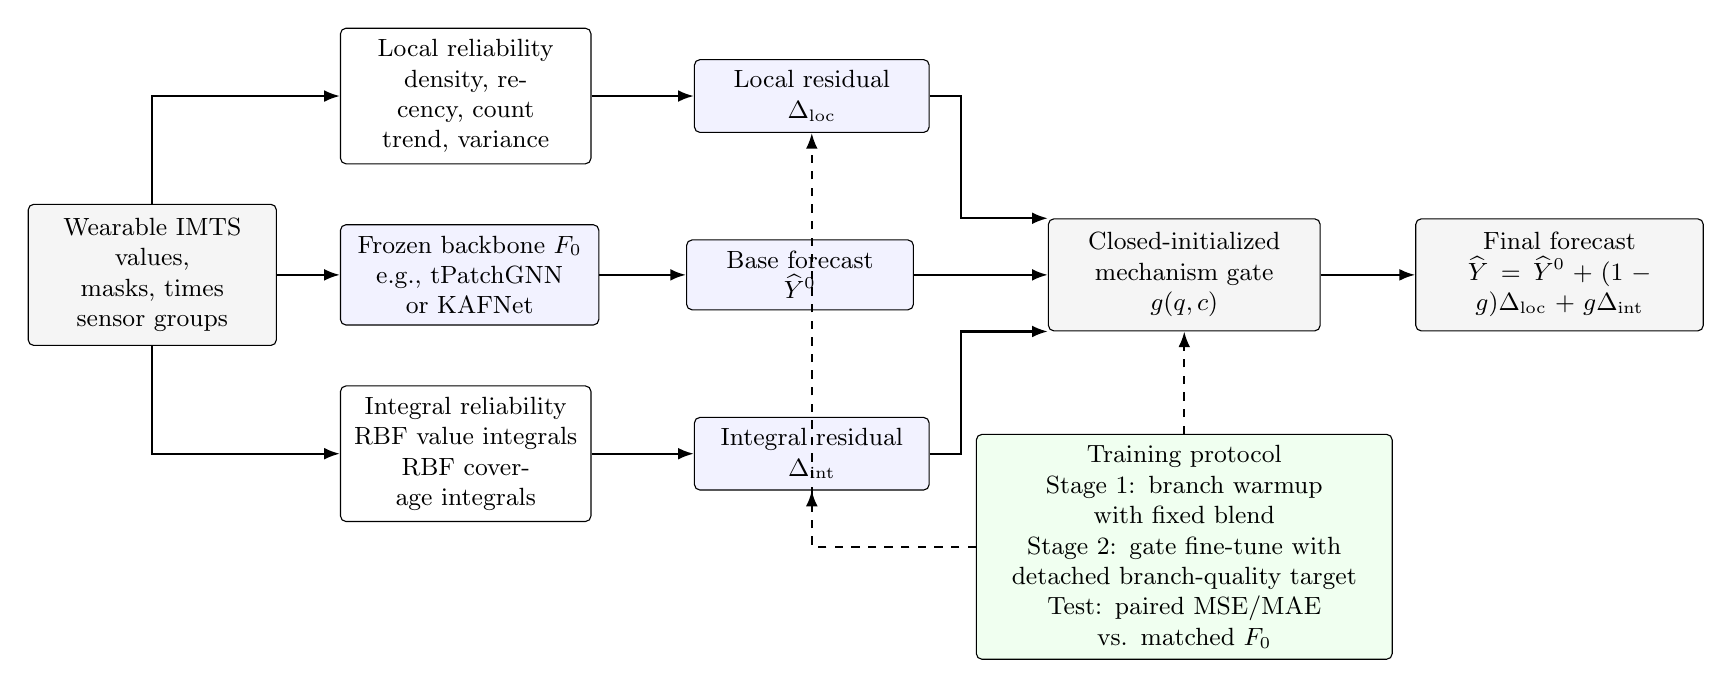
\begin{tikzpicture}[
  font=\small,
  box/.style={draw, rounded corners=2pt, align=center, minimum height=8mm, inner sep=4pt, fill=white},
  stage/.style={draw, rounded corners=2pt, align=center, minimum height=9mm, inner sep=5pt, fill=gray!8},
  op/.style={draw, rounded corners=2pt, align=center, minimum height=8mm, inner sep=4pt, fill=blue!5},
  arr/.style={-{Latex[length=2mm]}, thick},
  dasharr/.style={-{Latex[length=2mm]}, thick, dashed}
]
\node[stage, text width=28mm] (input) {Wearable IMTS\\values, masks, times\\sensor groups};
\node[op, right=8mm of input, text width=30mm] (base) {Frozen backbone \(F_0\)\\e.g., \baseT{} or \baseK{}};
\node[box, above right=5mm and 8mm of input, text width=29mm] (local) {Local reliability\\density, recency, count\\trend, variance};
\node[box, below right=5mm and 8mm of input, text width=29mm] (integral) {Integral reliability\\RBF value integrals\\RBF coverage integrals};
\node[op, right=13mm of local, text width=27mm] (locbranch) {Local residual\\\(\Delta_{\rm loc}\)};
\node[op, right=13mm of integral, text width=27mm] (intbranch) {Integral residual\\\(\Delta_{\rm int}\)};
\node[op, right=11mm of base, text width=26mm] (forecast) {Base forecast\\\(\widehat Y^0\)};
\node[stage, right=17mm of forecast, text width=31mm] (gate) {Closed-initialized\\mechanism gate\\\(g(q,c)\)};
\node[stage, right=12mm of gate, text width=33mm] (out) {Final forecast\\\(\widehat Y=\widehat Y^0+(1-g)\Delta_{\rm loc}+g\Delta_{\rm int}\)};
\node[box, below=13mm of gate, text width=50mm, fill=green!6] (train) {Training protocol\\Stage 1: branch warmup with fixed blend\\Stage 2: gate fine-tune with detached branch-quality target\\Test: paired MSE/MAE vs. matched \(F_0\)};

\draw[arr] (input) -- (base);
\draw[arr] (base) -- (forecast);
\draw[arr] (input) |- (local);
\draw[arr] (input) |- (integral);
\draw[arr] (local) -- (locbranch);
\draw[arr] (integral) -- (intbranch);
\draw[arr] (forecast) -- (gate);
\draw[arr] (locbranch.east) -- ++(4mm,0) |- (gate.north west);
\draw[arr] (intbranch.east) -- ++(4mm,0) |- (gate.south west);
\draw[arr] (gate) -- (out);
\draw[dasharr] (train) -- (gate);
\draw[dasharr] (train.west) -| (locbranch.south);
\draw[dasharr] (train.west) -| (intbranch.south);
\end{tikzpicture}
}
\caption{Overall view of \method.  A frozen IMTS backbone \(F_0\) provides the
level forecast; the paper instantiates this interface with \baseT{} and
\baseK{}.  Deployment-visible mechanism-state summaries feed local and integral
residual branches.  A closed-initialized gate selects the residual correction
per forecasted time--channel entry.  The training protocol is fixed: branch
warmup, gate fine-tuning, and paired test MSE/MAE against the matched \(F_0\)
checkpoint.}
\label{fig:architecture}
\end{figure*}

\subsection{Mechanism-State Residual Operator}

The method is built around a finite embedding of the wearable observation
measure.  For channel \(c\), define the deployment-visible empirical measure
\begin{equation}
\mu_c=\sum_{t\in\mathcal{H}} m_{t,c}\,\delta_{(t/T,\ x_{t,c})},
\end{equation}
where \(\mathcal{H}\) is the history window.  A value-only backbone mainly uses
observed values and times to form \(L\).  \method{} adds a separate
mechanism-state embedding
\begin{equation}
R_c=[\rho_{\rm loc}(\mu_c),\rho_{\rm int}(\mu_c)],
\end{equation}
where \(\rho_{\rm loc}\) contains low-order local moments and recency
statistics, while \(\rho_{\rm int}\) contains RBF kernel integrals of values
and coverage over the whole window.  This is the concrete approximation to
the mechanism state \(M=(V,R)\) in Theorem~\ref{thm:alias}.

The operator is constrained by three design rules.  First, it is
level-preserving: the output is the frozen \(F_0\) forecast plus a bounded
correction.  Second, it is mechanism-state only: the residual input is the
history observation measure, forecast time, and base prediction, not future
loss or dataset identity.  Third, it is branch-adaptive: recent local
mechanism cues and distributed integral value/coverage cues are trained as
separate residual mechanisms before the gate is allowed to select between them.
Together these rules turn the residual-frontier identity in
Theorem~\ref{thm:alias} into an implementable forecasting model: use mechanism
state only for the part that value-level patches cannot identify under squared
loss.

\textbf{\method{} operator contract.}
The operator is not an unrestricted adapter.  Its contract is:
\emph{inputs} are the frozen forecast \(\widehat Y^0=F_0(X)\), observed history
\(X\), forecast index \(q\), channel \(c\), and deployment-visible summaries of
\(\mu_c\); \emph{forbidden inputs} are future targets, test loss, validation
selection signals, dataset identity, and any update to \(F_0\);
\emph{invariant} is \(\widehat Y=\widehat Y^0\) at initialization; and
\emph{allowed action} is only a small additive mechanism-state residual.  This
contract is shared by \tpatchinst{} and \kafinst{} and is the reason the method
can be evaluated by exact paired gains against its own matched backbone.

The resulting operator has a soft-admission structure.  Each branch contains
its own negative-initialized residual gate, the
branch switch is also closed-initialized, and the objective penalizes residual
energy.  Thus the default prediction is exactly the strong backbone at
initialization, and the model must earn every correction through training
loss.  This matches the strong-backbone setting, where the remaining residual
frontier is small.

Soft admission has three nested levels in the implemented model:
\begin{equation}
\widehat Y
=\widehat Y^0+
\bigl(1-g(q,c)\bigr)\alpha_{\rm loc}\tilde\Delta_{\rm loc}
+g(q,c)\alpha_{\rm int}\tilde\Delta_{\rm int},
\end{equation}
with residual-energy regularization in the training objective.  The branch
amplitudes \(\alpha_{\rm loc},\alpha_{\rm int}\) decide whether a correction
should be applied; the switch \(g\) decides which mechanism scale should
dominate; the residual penalty keeps the whole correction close to zero unless
it consistently lowers forecasting loss.  Here \(\tilde\Delta_b\) denotes the
un-gated branch output and \(\alpha_b\) is defined in the branch module below.
This nested form is the main methodological difference from a plain additive
adapter.

\subsection{Mechanism-State Encoder}

For each variable, the local mechanism-state encoder computes the ten statistics
used in \texttt{MechanismSummaryEncoder}:
\begin{equation}
\begin{aligned}
\rho_{\rm loc} &= [d,\ d_{\rm rec},\ \log(1+\mathrm{count}),\ \bar t,\\
&\quad \sigma_t,\ t_{\rm rec},\ \bar x,\ \sigma_x,\ x_{\rm rec},\ x_{\rm rec}-x_{\rm early}]
\end{aligned}
\end{equation}
These are exactly the features in the implementation.  They capture how much
of a channel was observed, whether it was recently observed, how dispersed its
observation times are, and whether recent values differ from early values.

The integral encoder appends RBF value and coverage integrals.  These are a
small kernel-mean embedding of \(\mu_c\), chosen because wearable reliability
can depend on distributed coverage over the whole history rather than only on
the last observation.  For RBF center \(c_m\), width \(w\), mask \(m_t\), and
value \(x_t\),
\begin{equation}
\begin{aligned}
I_m^x &=
\frac{\sum_t \omega_m(t)m_t x_t}
     {\sum_t \omega_m(t)m_t+\epsilon},\\
I_m^m &=
\frac{\sum_t \omega_m(t)m_t}
     {\sum_t \omega_m(t)+\epsilon},
\quad
\omega_m(t)=e^{-(t-c_m)^2/(2w^2)} .
\end{aligned}
\end{equation}
The number of centers, width, and MLP size are fixed by the registered
experimental protocol.

\subsection{Local and Integral Branches}

Both branches receive a reliability embedding \(r_c^b\), forecast-time
embedding \(e_q\), and the base prediction value
\(\widehat{Y}^{0}_{q,c}\).  For branch
\(b\in\{\mathrm{loc},\mathrm{int}\}\),
\begin{equation}
\Delta_b(q,c)
=
\alpha_b(q,c)
\cdot
h_b([r_c^b,e_q,\widehat{Y}^{0}_{q,c}]).
\end{equation}
where \(\alpha_b(q,c)=\sigma(u_b^\top[r_c^b,e_q])\) is a branch-level
admission gate.
The local branch uses only \(\rho_{\rm loc}\).  The integral branch uses
\(\rho_{\rm loc}\) plus RBF value/coverage integrals.  Both branch gates have
negative bias initialization, so their initial residuals are small.

This branch-level gate is the first residual-admission layer: it lets a
mechanism feature help where predictive without forcing every time--channel
entry to be corrected.  The soft-admission ablation shows that the gain is not
tied to one gate hyperparameter; \method{} therefore keeps both local and
integral mechanism summaries and learns a sample-wise switch above them.

\subsection{Mechanism Gate}

The mechanism gate chooses between local and integral correction:
\begin{equation}
g(q,c)=\sigma\big(s(r_c^{\rm sw},e_q,\widehat{Y}^{0}_{q,c},
|\Delta_{\rm loc}(q,c)-\Delta_{\rm int}(q,c)|)\big).
\end{equation}
The disagreement term is part of the implementation.  If the branches agree,
the choice has low risk; if they disagree, the gate must use mechanism state
to decide whether local recency, value level, or integral coverage is more
predictive.

Training has two stages.  Stage 1 warms up both branches with a fixed equal
blend, independent of the learned switch.  Stage 2 learns \(g\) with a
small boundary penalty \(g(1-g)\) and a detached branch-quality target.  The
target compares the training losses of local and integral branch predictions;
it uses labels only during training.  At deployment, the gate uses only
history \(X\), forecast time, and the base forecast.

The gate is the registered default.  Its role is stable closed initialization
and interpolation between local and integral mechanism corrections.
Table~\ref{tab:branch-ablation} reports the effects of removing warmup,
boundary regularization, residual \(L_2\), or the supervised target.  The core method is the
mechanism-state residual operator; soft admission places it on a strong
backbone.

Concretely, let
\(\ell_{\rm loc}=(\widehat{Y}_{\rm loc}-Y)^2\) and
\(\ell_{\rm int}=(\widehat{Y}_{\rm int}-Y)^2\) during training.  The detached
gate target in the implementation is a softened branch comparison:
\begin{equation}
T=\sigma\!\left(
\frac{\ell_{\rm loc}-\ell_{\rm int}-m}
{\tau(\ell_{\rm loc}+\ell_{\rm int})+\epsilon}
\right),
\end{equation}
weighted by confidence \(2|T-0.5|\) with a minimum-confidence threshold.
This gives the switch direct supervision about which branch is better on a
training example, while preventing test-time label leakage because \(T\) is not
available or used at deployment.

\subsection{Level-Preserving Residual Operator}

The implemented operator is level-preserving: the original \(F_0\) forecast is
always present as an additive anchor, and the learned module can only predict a
bounded correction.  This matters for the target suite.  Wearable windows have
large value-level dynamics driven by activity intensity.  The residual module
models the mechanism-dependent residual left after backbone forecasting.  We therefore
distinguish three paths:
\[
\widehat Y^0=F_0(X),\qquad
\widehat Y_{\rm loc}=\widehat Y^0+\Delta_{\rm loc},\qquad
\widehat Y_{\rm int}=\widehat Y^0+\Delta_{\rm int}.
\]
Stage-1 warmup trains the two residual paths under a fixed blend so that each
branch learns a meaningful correction before the gate can prefer one.  Stage-2
gate training then solves a branch-selection problem in residual space.  The negative branch biases and
residual \(L_2\) penalty implement the finite-sample implication of
Proposition~\ref{prop:residual-value}: when the frontier is weak, the learned
residual stays close to zero and the output remains close to the backbone.

\textbf{Train/deploy separation.}
The branch-quality target \(T\) is a supervised training signal, analogous to
ordinary labels in a forecasting loss.  It is computed on training
examples to shape the gate.  The deployed gate receives
\((R_{\rm loc},R_{\rm int},e_q,\widehat Y^0,\Delta_{\rm loc},\Delta_{\rm int})\)
and uses no target labels, validation loss, test loss, or realized branch loss.

\textbf{Backbone-preserving regime.}
\method{} treats the chosen \(F_0\) as the value-dynamics expert and learns
only the mechanism-state residual.  The model is evaluated in the regime where
strong IMTS backbones already give competitive value forecasts, while wearable
mechanism states still split residual behavior inside value-level strata.

\subsection{Training Objective}

The training objective is
\[
\begin{aligned}
\mathcal{L}=&\ \mathrm{MSE}(\widehat{Y},Y)
+\lambda_{\rm res}\|\Delta_{\rm RAMS}\|_2^2\\
&+\lambda_{\rm bd}\E[g(1-g)]
+\lambda_{\rm sup}\mathcal{L}_{\rm gate}.
\end{aligned}
\]
All numerical values for the penalties, gate initialization, and residual
architecture are listed in the experimental protocol.
The ablation disables these ingredients one at a time to test whether the
forecasting improvement comes from the mechanism-state residual itself or from a
particular admission hyperparameter.

\begin{algorithm}[t]
\caption{Registered \method{} training and inference}
\label{alg:ramstpatch}
\small
\begin{algorithmic}[1]
\REQUIRE training windows \(X,Y\), validation split, test split, trained or
trainable backbone checkpoint \(F_0\)
\STATE Train or load a public IMTS backbone under the shared conversion; keep
the matched \(F_0\) checkpoint for each dataset and seed.
\STATE Initialize \method{} with \(F_0\) as the frozen level predictor; freeze
all \(F_0\) parameters.
\STATE Build local and integral mechanism-state encoders from deployment-visible
history statistics.
\STATE Stage 1: train \(\Delta_{\rm loc}\) and \(\Delta_{\rm int}\) with fixed
blend \(g=0.5\).
\STATE Stage 2: train learned gate \(g\), residual loss, residual shrinkage,
boundary penalty, and detached branch-quality loss.
\STATE Select no branch per dataset: deploy the registered learned gate for
all target datasets.
\STATE At inference, compute \(\widehat{Y}^{0}=F_0(X)\), compute
\(\Delta_{\rm RAMS}\), and output Eq.~\eqref{eq:main-model}; report paired
test MSE/MAE against the same \(F_0\).
\end{algorithmic}
\end{algorithm}

The residual sees protocol-valid mechanism state \(M\), uses local/integral
branches, and is admitted through the registered closed-initialized gate.  The
same default is used for every target dataset.

\section{Experiments}

\subsection{Experimental Questions}

The experiments are designed around the generic \(F_0+\Delta_{\rm RAMS}\)
interface.  \textbf{RQ1:} Which reproduced public IMTS backbones are strong
under the same wearable forecasting conversion?  \textbf{RQ2:} Does
\tpatchinst{} improve a matched frozen \baseT{} checkpoint on ordinary test
MSE/MAE?  \textbf{RQ3:} Does \kafinst{} improve a matched frozen \baseK{}
checkpoint under the same residual protocol?  \textbf{RQ4:} Which parts of the
mechanism-state operator matter: branch capacity, local/integral scale, real
alignment, or value/reliability summaries?  \textbf{RQ5:} Is the
mechanism-state aliasing frontier measurable in real wearable data?

\subsection{Datasets, Backbones, and Instances}

We evaluate on MHEALTH, OPPORTUNITY, and PAMAP2.  These datasets form the
target group-asynchronous wearable suite.  The public baseline scan includes
APNResearch, \baseK{}, GraFITi, and \baseT{} under the same data conversion and
metric code.  \baseT{} is strongest on all three target datasets, so the first
instantiation, \tpatchinst{}, freezes the matched \baseT{} checkpoint and
trains the \method{} operator on top of it.  The forecasting conversion uses
history/horizon/patch lengths
\((250,50,25)\), \((300,60,30)\), and \((500,100,50)\) for MHEALTH,
OPPORTUNITY, and PAMAP2, respectively, with 23, 64, and 37 observed channels.
The \baseK{} instantiation, \kafinst{}, freezes \baseK{} and keeps the same
mechanism-state residual operator, optimizer, split rule, metric code, and
closed-gate default.  The \baseK{} paired evaluation covers HumanActivity,
MHEALTH, OPPORTUNITY, and PAMAP2, including all three main-suite datasets.
This setting tests whether \method{} is a backbone-level residual principle
rather than a \baseT{}-specific module.

For each dataset, seed, and backbone, \method{} is evaluated against the exact
matched \(F_0\) checkpoint under the same split, loss, horizon, and metric
implementation.  Reported gains are paired forecasting gains over that matched
frozen checkpoint.

\begin{table}[t]
\centering
\caption{Shared-protocol public baseline scan and compact absolute performance
on the main wearable suite.  Entries are MSE/MAE; lower is better.}
\label{tab:baseline-scan}
\footnotesize
\resizebox{\columnwidth}{!}{%
\begin{tabular}{lcccccc}
\toprule
Dataset & APN & \baseK{} & GraFITi & \baseT{} & \tpatchinst{} & \kafinst{} \\
\midrule
MHEALTH & .761/.484 & .751/.478 & .736/.464 & .705/.446 & \textbf{.696/.438} & .718/.452 \\
OPPORTUNITY & .823/.656 & .848/.676 & .834/.664 & .733/.594 & \textbf{.718/.585} & .754/.612 \\
PAMAP2 & .795/.504 & .818/.525 & .793/.509 & .756/.464 & \textbf{.753/.460} & .770/.485 \\
\bottomrule
\end{tabular}
}
\end{table}

\subsection{Protocol}

For every seed, dataset, and backbone instance, we first train or load the
matched frozen checkpoint \(F_0\) with the public baseline protocol.  For
\tpatchinst{}, we report two paired tiers.  The 4-epoch tier is the registered
scan/ablation protocol because it trains all public baselines and all
\method{} branches under one manifest.  The 8-epoch tier is the
stronger-backbone confirmation: it retrains the \baseT{} checkpoint longer and
repeats the same frozen-backbone gate procedure.  For \kafinst{}, we report the
available three-seed frozen-\baseK{} paired rows on HumanActivity, MHEALTH,
OPPORTUNITY, and PAMAP2.  In all cases \method{} is
trained for three residual epochs with MSE loss and frozen \(F_0\).  Batch size
follows the registered manifest; for the KAFNet confirmation it is 16 on
HumanActivity and 32 on MHEALTH, OPPORTUNITY, and PAMAP2.  The UCI wearable runs use collate\_fn\_patch and dataset-specific patch lengths: 25 for
MHEALTH, 30 for OPPORTUNITY, and 50 for PAMAP2.  The model is evaluated on
the same test split as its own base checkpoint.  No test metric is used to
train the gate.

The processed wearable records use a fixed record-order split: 81\% train,
9\% validation, and 10\% test, with no shuffling.  Windows are generated with
the repository activity-chunk stride of 4000 raw time units.  Continuous
channels are standardized once by feature-wise observed-value mean and standard
deviation before applying the group-asynchronous mask; every baseline and
\method{} run consumes the same processed tensors.  All wearable runs use Adam,
learning rate \(10^{-3}\), delayed-step decay, validation interval 1, patience
2 in the registered RAMS runs, and one training iteration per seed.

Both tiers use the same residual architecture.  The mechanism-state encoder
computes the ten local statistics in Sec.~\ref{sec:method}, appends six RBF
value/coverage integrals with width 0.18, and passes the local and integral
vectors through two-layer GELU MLPs with layer normalization.  Stage 1 uses a
fixed 0.5 blend for branch warmup.  Stage 2 uses residual penalty
\(\lambda_{\rm res}=10^{-4}\), branch gate initialization \(-3.0\), switch
initialization \(-2.5\), boundary penalty
\(\lambda_{\rm bd}=2\times10^{-4}\), and supervised gate weight \(0.02\).

The default model is fixed before aggregation: the closed-initialized
\texttt{gate}.  The ablations test which parts of the admission procedure affect
the result.  The target metric is ordinary test MSE/MAE.

\textbf{Aggregation rule.}
All averages are computed over the registered dataset--seed list in the
experiment manifest.  A seed contributes a paired row only if both the matched
\(F_0\) checkpoint and the \method{} checkpoint finish under the same split,
horizon, and metric implementation.  The gate is fixed before reading aggregate
results, while
no-warmup, open-gate, no-residual-\(L_2\), no-gate-target, and no-boundary
rows are soft-admission ablations.  Public baselines are trained under the
same conversion before any \method{} aggregate is interpreted.

\begin{table}[t]
\centering
\caption{Registered forecasting protocol.  These settings match the experiment
script and are kept fixed across the target suite.}
\label{tab:protocol}
\small
\resizebox{\columnwidth}{!}{%
\begin{tabular}{ll}
\toprule
Item & Setting \\
\midrule
Backbone interface & frozen \(F_0\) \\
Backbone update & frozen \\
Public baselines & APNResearch/\baseK{}/GraFITi/\baseT{} \\
Backbone instances & \tpatchinst{} on \baseT{}; \kafinst{} on \baseK{} \\
Residual module & shared \method{} mechanism-state operator \\
Default variant & learned \texttt{gate} \\
Residual epochs & 3 \\
Base epochs & 4 scan/ablation; 8 strong confirmation \\
Loss & MSE \\
Batch size & manifest value; KAFNet 16/32 \\
Optimizer / LR & Adam / \(10^{-3}\) \\
Split & 81\% train, 9\% validation, 10\% test \\
Patch length & 25/30/50 for MHEALTH/OPP/PAMAP2 \\
History/horizon & 250/50, 300/60, 500/100 \\
RBF centers / width & 6 / 0.18 \\
Residual penalties & \(10^{-4}\) residual, \(2{\times}10^{-4}\) boundary \\
Gate initialization & branch \(-3.0\), switch \(-2.5\) \\
Gate supervision & weight 0.02, fixed 0.5 warmup blend \\
Seeds & three paired seeds per reported dataset \\
Pairing & exact matched \(F_0\) checkpoint per dataset--seed \\
Metrics & test MSE, test MAE \\
\bottomrule
\end{tabular}
}
\end{table}

\textbf{Implementation and overhead.}
\method{} adds no graph construction, raw-event attention, or backbone update.
Its overhead is a mechanism-state scan, six RBF value/coverage integrals, and
two small MLP residual branches.  For \(C\) channels, history length \(T\),
horizon \(H\), \(M=6\) RBF centers, and residual width \(d\), the additional
work is \(O(CT+CTM+CHd^2)\), while the backbone graph or attention computation
is unchanged.

\subsection{Backbone-Parallel Paired Forecasting Results: RQ1--RQ3}

\begin{table*}[t]
\centering
\caption{\tpatchinst{} registered 4-epoch paired scan results.  \method{} uses one
fixed default: the learned gate.  It improves the strongest reproduced public
IMTS backbone under the shared protocol (\baseT{}) on all average MSE/MAE
comparisons in the main wearable suite.}
\label{tab:main}
\small
\resizebox{\textwidth}{!}{%
\begin{tabular}{lccccccccc}
\toprule
Dataset & \(n\) & \baseT{} MSE & \tpatchinst{} MSE & MSE gain & MSE wins & \baseT{} MAE & \tpatchinst{} MAE & MAE gain & MAE wins \\
\midrule
MHEALTH & 3 & 0.705 & 0.696 & 1.19\% & 3/3 & 0.446 & 0.438 & 1.81\% & 3/3 \\
OPPORTUNITY & 3 & 0.733 & 0.718 & 2.11\% & 3/3 & 0.594 & 0.585 & 1.56\% & 3/3 \\
PAMAP2 & 3 & 0.756 & 0.753 & 0.33\% & 3/3 & 0.464 & 0.460 & 0.78\% & 3/3 \\
\bottomrule
\end{tabular}
}
\end{table*}

Table~\ref{tab:baseline-scan} answers RQ1 and separates absolute performance
from backbone transfer.  \baseT{} is the strongest reproduced public IMTS
backbone under the shared conversion, \tpatchinst{} gives the lowest
main-suite MSE/MAE, and \kafinst{} shows the same operator improves a different
frozen backbone.  Table~\ref{tab:main} answers RQ2 for the \baseT{} instance.  A
single \method{} gate improves the matched \baseT{} checkpoint on every
dataset-metric average.  Across the nine dataset--seed pairs, \tpatchinst{}
wins eight times on MSE and eight times on MAE.  Because the comparison is
paired against the exact matched checkpoint modified by \method{}, the gains
measure residual forecasting value rather than differences in splits, horizons,
or preprocessing.

\begin{table}[t]
\centering
\caption{Paired aggregate evidence for the 4-epoch registered protocol over
the nine dataset--seed pairs.  Bootstrap \(p\) is one-sided
\(\Pr(\bar g\le0)\) from paired resampling; sign \(p\) is the exact one-sided
sign test.}
\label{tab:ci}
\small
\resizebox{\columnwidth}{!}{%
\begin{tabular}{lcccc}
\toprule
Metric & Mean gain & 95\% boot CI & Wins & \(p_{\rm boot}/p_{\rm sign}\) \\
\midrule
MSE & 1.210\% & \([0.330, 2.110]\) & 9/9 & \(<0.001/0.002\) \\
MAE & 1.383\% & \([0.780, 1.810]\) & 9/9 & \(<0.001/0.002\) \\
\bottomrule
\end{tabular}
}
\end{table}

Table~\ref{tab:ci} reports paired uncertainty and mean gains.  The
registered three-seed protocol is paired at the checkpoint level: each
\tpatchinst{} model is compared with the exact \baseT{} checkpoint it modifies.
The evidence
has two stable positives and one smaller-margin positive.  MHEALTH and PAMAP2
are positive for both metrics in every seed, with positive bootstrap intervals
within the three-seed rows.  OPPORTUNITY improves in mean, with MSE gains
ranging from \(-0.79\%\) to \(1.50\%\) and MAE gains from \(-0.03\%\) to
\(0.49\%\).  At the suite level, the nine paired rows give positive aggregate
evidence for both MSE and MAE.

\begin{table}[H]
\centering
\caption{\tpatchinst{} 8-epoch strong-backbone confirmation.  Entries show
paired base-to-\method{} values, gain percentages, and seed wins.}
\label{tab:strong}
\footnotesize
\resizebox{\columnwidth}{!}{%
\begin{tabular}{lccccc}
\toprule
Dataset & MSE base\(\to\)ours & Gain & Wins & MAE base\(\to\)ours & Gain/Wins \\
\midrule
MHEALTH & 0.701129\(\to\)0.693718 & 1.048\% & 3/3 & 0.443561\(\to\)0.435146 & 1.877\% / 3/3 \\
OPPORTUNITY & 0.708311\(\to\)0.703887 & 0.620\% & 2/3 & 0.575071\(\to\)0.572392 & 0.466\% / 3/3 \\
PAMAP2 & 0.756257\(\to\)0.752854 & 0.449\% & 3/3 & 0.467224\(\to\)0.460352 & 1.460\% / 3/3 \\
\bottomrule
\end{tabular}
}
\end{table}

Table~\ref{tab:strong} reports the 8-epoch strong-backbone confirmation for
RQ2.  The stronger 8-epoch \baseT{} lowers the raw
backbone error on all three datasets, yet the same frozen-backbone gate remains
positive on all six average comparisons, with 8/9 MSE and 9/9 MAE seed wins.
The effect sizes shrink as the base predictor absorbs more of the residual
frontier, while the direction remains consistent.

\subsection{\baseK{} Backbone Results: RQ3}

\begin{table}[t]
\centering
\caption{\kafinst{} paired results.  The frozen backbone is \baseK{}, while the
same mechanism-state residual gate, loss, split, and metric code are used.}
\label{tab:kafnet-confirm}
\footnotesize
\resizebox{\columnwidth}{!}{%
\begin{tabular}{lccccc}
\toprule
Dataset & \(n\) & \baseK{} MSE/MAE & \kafinst{} MSE/MAE & MSE gain & MAE gain \\
\midrule
HumanActivity & 3 & 0.044 / 0.121 & 0.042 / 0.115 & 4.08\% & 5.14\% \\
MHEALTH & 3 & 0.763 / 0.491 & 0.718 / 0.452 & 5.85\% & 7.89\% \\
OPPORTUNITY & 3 & 0.848 / 0.678 & 0.754 / 0.612 & 11.10\% & 9.66\% \\
PAMAP2 & 3 & 0.816 / 0.525 & 0.770 / 0.485 & 5.63\% & 7.62\% \\
\bottomrule
\end{tabular}
}
\end{table}

\begin{table}[t]
\centering
\caption{\kafinst{} paired aggregate evidence over all twelve completed
dataset--seed rows.  Bootstrap \(p\) is one-sided paired resampling; sign
\(p\) is the exact one-sided sign test.}
\label{tab:kafnet-ci}
\footnotesize
\resizebox{\columnwidth}{!}{%
\begin{tabular}{lcccc}
\toprule
Metric & Mean gain & 95\% boot CI & Wins & \(p_{\rm boot}/p_{\rm sign}\) \\
\midrule
MSE & 6.665\% & \([4.080, 11.100]\) & 12/12 & \(<10^{-5}/2.44{\times}10^{-4}\) \\
MAE & 7.578\% & \([5.140, 9.660]\) & 12/12 & \(<10^{-5}/2.44{\times}10^{-4}\) \\
\bottomrule
\end{tabular}
}
\end{table}

Table~\ref{tab:kafnet-confirm} answers RQ3.  HumanActivity, MHEALTH,
OPPORTUNITY, and PAMAP2 are all three-seed \baseK{} paired evaluations, and
\kafinst{} wins all paired seeds on both MSE and MAE over the matched frozen
\baseK{} base.  The main-suite KAFNet rows are especially strong: MHEALTH
improves by 4.40\%/5.82\%, OPPORTUNITY by 11.73\%/9.99\%, and PAMAP2 by
5.63\%/6.97\% in MSE/MAE.  Table~\ref{tab:kafnet-ci} adds the aggregate paired
uncertainty: all twelve rows are positive, with bootstrap intervals strictly
above zero.  Together,
Tables~\ref{tab:main} and \ref{tab:kafnet-confirm} show the intended use of
\method{}: the same mechanism-state residual operator can be attached to
different trained IMTS backbones, and the reported gain is always measured
against the exact frozen checkpoint it modifies.

\textbf{Dataset-level results.}
For \tpatchinst{}, MHEALTH and PAMAP2 are the stable positives: both win all
three seeds on both metrics in the 4-epoch protocol, and both remain positive
after the backbone is strengthened.  OPPORTUNITY has positive mean gains with smaller seed-level
margins and one negative MSE edge case in the scan protocol.  The diagnostic in
Table~\ref{tab:alias} reports the residual-variance share used to quantify the
observed mechanism-state frontier in each dataset.

\subsection{Soft-Admission and Mechanism Controls: RQ4}

Table~\ref{tab:branch-ablation} separates the branch choices from the input
state controls.  Local-only and integral-only residuals are already positive,
confirming that both short-range mechanism summaries and distributed
coverage/value integrals carry usable residual information.  The registered
gate has the best suite-average MSE/MAE gain, so we keep it as the fixed
deployment rule rather than selecting branches per dataset.

\begin{table}[H]
\centering
\caption{Branch/gate ablation aggregated over the nine registered
\baseT{} dataset--seed pairs.  Entries are paired gain percentages and seed
wins over the same frozen checkpoints.}
\label{tab:branch-ablation}
\footnotesize
\begin{tabular}{lcccc}
\toprule
Variant & MSE gain & MSE wins & MAE gain & MAE wins \\
\midrule
Local & 0.804 & 9/9 & 1.343 & 8/9 \\
Integral & 0.843 & 9/9 & 1.397 & 8/9 \\
Fixed mix & 0.835 & 9/9 & 1.400 & 8/9 \\
Gate & \textbf{0.851} & 8/9 & \textbf{1.482} & 8/9 \\
Conservative gate & 0.798 & 8/9 & 1.471 & 8/9 \\
\bottomrule
\end{tabular}
\end{table}

We further run input controls that keep the same frozen \baseT{} checkpoint,
training schedule, and gate, while replacing the residual input state.  The
\emph{value-only} control removes mask density, recency, effective counts, time
span, and coverage integrals; the \emph{reliability-only} control removes
value moments and value integrals; the \emph{shuffled} control batch-rolls the
mechanism state so that marginal scale remains but sample alignment is broken.
Table~\ref{tab:state-control} shows two facts.  First, value summaries,
reliability summaries, and residual capacity each contribute to the residual
operator.  Second, the full aligned state is best or essentially tied on MHEALTH
and PAMAP2, while OPPORTUNITY has smaller margins.  The shuffled control
preserves residual-input scale but breaks the sample-specific
\(M\)-to-residual link in Theorem~\ref{thm:alias}.

\begin{table}[H]
\centering
\caption{Mechanism-state controls. Entries are paired MSE/MAE gain percentages
over the same frozen \baseT{} checkpoint.}
\label{tab:state-control}
\footnotesize
\resizebox{\columnwidth}{!}{%
\begin{tabular}{lcccc}
\toprule
Dataset & Real & Value & Reliab. & Shuffled \\
\midrule
MHEALTH & \textbf{1.346/2.082} & 1.202/1.976 & 0.976/1.833 & 0.991/1.870 \\
OPPORTUNITY & 0.524/\textbf{0.214} & \textbf{0.715}/0.161 & 0.600/-0.055 & 0.596/-0.060 \\
PAMAP2 & \textbf{0.683}/2.152 & 0.654/\textbf{2.165} & 0.435/1.422 & 0.425/1.387 \\
\bottomrule
\end{tabular}
}
\end{table}

\subsection{Mechanism-State Aliasing Diagnostic: RQ5}

We also estimate whether the theory's mechanism-state frontier exists before
training the neural residual.  For each wearable window, we compute a
deployment-visible value-level summary \(L\) and mechanism summary \(M=(V,R)\).
We then discretize \(L\) into value-level strata and ask whether mechanism
bins split the future level residual inside the same value stratum.  This is
the empirical counterpart of Theorem~\ref{thm:alias} and
Proposition~\ref{prop:diagnostic}: if mechanism state does not change the
conditional residual after value matching, the coarse frontier statistic should
be near zero.

The diagnostic is an ANOVA-style coarse frontier statistic
\begin{equation}
D_{\rm split}
=
\sum_\ell \widehat p(\ell)
\sum_r \widehat p(r\mid \ell)
\|\widehat\mu_{\ell,r}-\widehat\mu_{\ell}\|_2^2,
\end{equation}
where \(\widehat\mu_{\ell,r}\) is the mean future residual in value stratum
\(\ell\) and mechanism bin \(r\).  We report both \(D_{\rm split}\) and its
percentage of residual variance.  Because the value state is binned rather
than observed exactly, this is a coarse proxy for \(\mathcal{F}_M(F_0)\).  It is
computed after model evaluation and checks whether mechanism state splits
value-matched residuals in the target suite.

\begin{table}[H]
\centering
\caption{Mechanism-state aliasing diagnostic.  After value matching,
mechanism bins explain nonzero residual variation.}
\label{tab:alias}
\small
\resizebox{\columnwidth}{!}{%
\begin{tabular}{lcccc}
\toprule
Dataset & \(n\) & \(D_{\rm split}\) & Residual-var. share & Mean gap \\
\midrule
MHEALTH & 2021 & \(5.34{\times}10^{-3}\) & 0.789\% & 0.060 \\
OPPORTUNITY & 785 & \(8.17{\times}10^{-3}\) & 1.522\% & 0.087 \\
PAMAP2 & 902 & \(6.23{\times}10^{-3}\) & 1.024\% & 0.069 \\
\bottomrule
\end{tabular}
}
\end{table}

The diagnostic answers RQ4 directly.  All three datasets have a nonzero
value-stratified mechanism split, accounting for roughly 0.79--1.52\% of
residual variance.  These are small numbers, which is consistent with the
fact that \baseT{} is already a strong patch-graph forecaster; nevertheless
they are of the same order as the paired MSE gains in
Table~\ref{tab:main}.  This closes the theory-to-experiment loop:
deployment-visible mechanism state splits value-matched residuals, and a
compact nonlinear mechanism residual recovers a portion of that frontier in
forecasting MSE/MAE.

\subsection{Reproducibility and Diagnostics}

The registered 4-epoch per-seed signs match the dataset-level reading:
MHEALTH and PAMAP2 are positive in every paired seed on both metrics, while
OPPORTUNITY has one negative MSE seed and one near-zero negative MAE seed.  The
diagnostic in Table~\ref{tab:alias} uses five value-summary quantile bins,
three mechanism-summary quantile bins, and a minimum cell size of eight
windows.  All reported tables are constructed from paired CSV summaries
produced by the same forecasting pipeline: the same dataset, seed, split,
horizon, metric implementation, and matched frozen \(F_0\) checkpoint are used
for every gain.  The baseline scan is aggregated before any \method{} rows;
Tables~\ref{tab:main}, \ref{tab:ci}, \ref{tab:strong}, and
\ref{tab:kafnet-confirm} use the corresponding paired rows; and
Tables~\ref{tab:branch-ablation}--\ref{tab:alias} change only the residual
variant, residual input, or diagnostic readout.

\section{Conclusion}

In this paper, we proposed \method{}, a mechanism-state residual operator
for forecasting group-asynchronous wearable IMTS.  The key idea is to preserve
a trained IMTS backbone as the value-level predictor and construct a small
residual correction from deployment-visible mechanism state.  The
mechanism-state aliasing identity explains when such a correction can reduce
forecasting risk: if value-matched wearable windows have different
mechanism-conditioned residual means, a value-only patch state leaves a
recoverable residual frontier.

\method{} implements this idea with local reliability summaries, integral
value/coverage summaries, and a closed-initialized gate.  Instantiated on two
frozen backbones, \tpatchinst{} improves matched \baseT{} checkpoints on
MHEALTH, OPPORTUNITY, and PAMAP2 in both 4-epoch and 8-epoch protocols, while
\kafinst{} improves matched \baseK{} checkpoints on HumanActivity, MHEALTH,
OPPORTUNITY, and PAMAP2, winning all 12 reported paired dataset--seed rows on
both metrics.  Ablations, mechanism-state controls, and aliasing diagnostics
show that the gains come from aligned wearable mechanism information rather
than generic residual capacity.

\begin{thebibliography}{99}

\bibitem{grud}
Z. Che, S. Purushotham, K. Cho, D. Sontag, and Y. Liu.
Recurrent neural networks for multivariate time series with missing values.
\emph{Scientific Reports}, 2018.

\bibitem{brits}
W. Cao, D. Wang, J. Li, H. Zhou, L. Li, and Y. Li.
BRITS: Bidirectional recurrent imputation for time series.
\emph{NeurIPS}, 2018.

\bibitem{latentode}
Y. Rubanova, R. T. Q. Chen, and D. Duvenaud.
Latent ordinary differential equations for irregularly-sampled time series.
\emph{NeurIPS}, 2019.

\bibitem{seft}
M. Horn, M. Moor, C. Bock, B. Rieck, and K. Borgwardt.
Set functions for time series.
\emph{ICML}, 2020.

\bibitem{mtan}
S. Shukla and B. Marlin.
Multi-time attention networks for irregularly sampled time series.
\emph{ICLR}, 2021.

\bibitem{rubin}
D. B. Rubin.
Inference and missing data.
\emph{Biometrika}, 63(3):581--592, 1976.

\bibitem{grafiti}
V. K. Yalavarthi, K. Madhusudhanan, R. Scholz, N. Ahmed, J. Burchert,
S. Jawed, S. Born, and L. Schmidt-Thieme.
GraFITi: Graphs for forecasting irregularly sampled time series.
\emph{AAAI}, 2024.

\bibitem{tpatchgnn}
W. Zhang, C. Yin, H. Liu, X. Zhou, and H. Xiong.
Irregular multivariate time series forecasting: A transformable patching graph
neural networks approach.
\emph{ICML}, 2024.

\bibitem{life}
Z.-Y. Zhang, S.-Q. Zhang, Y. Jiang, and Z.-H. Zhou.
LIFE: Learning individual features for multivariate time series prediction
with missing values.
\emph{IEEE BigData}, 2021.

\bibitem{jointlocalglobal}
X. Tang, H. Yao, Y. Sun, C. Aggarwal, P. Mitra, and S. Wang.
Joint modeling of local and global temporal dynamics for multivariate time
series forecasting with missing values.
\emph{AAAI}, 2020.

\bibitem{informer}
H. Zhou, S. Zhang, J. Peng, S. Zhang, J. Li, H. Xiong, and W. Zhang.
Informer: Beyond efficient transformer for long sequence time-series
forecasting.
\emph{AAAI}, 2021.

\bibitem{autoformer}
H. Wu, J. Xu, J. Wang, and M. Long.
Autoformer: Decomposition transformers with auto-correlation for long-term
series forecasting.
\emph{NeurIPS}, 2021.

\bibitem{timesnet}
H. Wu, T. Hu, Y. Liu, H. Zhou, J. Wang, and M. Long.
TimesNet: Temporal 2D-variation modeling for general time series analysis.
\emph{ICLR}, 2023.

\bibitem{patchtst}
Y. Nie, N. H. Nguyen, P. Sinthong, and J. Kalagnanam.
A time series is worth 64 words: Long-term forecasting with transformers.
\emph{ICLR}, 2023.

\bibitem{mtgnn}
Z. Wu, S. Pan, G. Long, J. Jiang, and C. Zhang.
Connecting the dots: Multivariate time series forecasting with graph neural
networks.
\emph{KDD}, 2020.

\bibitem{kafnet}
X. Liu, W. Liu, Z. Li, J. Chen, and H. Chen.
Canonical pre-alignment for irregularly sampled multivariate time series
forecasting.
\emph{AAAI}, 2026.

\bibitem{lara}
O. D. Lara and M. A. Labrador.
A survey on human activity recognition using wearable sensors.
\emph{IEEE Communications Surveys \& Tutorials}, 15(3):1192--1209, 2013.

\bibitem{mhealth}
O. Banos, C. Villalonga, R. Garcia, A. Saez, M. Damas, J. A. Holgado,
S. Lee, H. Pomares, and I. Rojas.
Design, implementation and validation of a novel open framework for agile
development of mobile health applications.
\emph{Biomedical Engineering Online}, 2015.

\bibitem{opportunity}
D. Roggen, A. Calatroni, M. Rossi, T. Holleczek, K. Forster, G. Troster,
P. Lukowicz, D. Bannach, G. Pirkl, A. Ferscha, J. Doppler, C. Holzmann,
M. Kurz, G. Holl, R. Chavarriaga, H. Sagha, H. Bayati, M. Creatura, and
J. del R. Millan.
Collecting complex activity datasets in highly rich networked sensor
environments.
\emph{INSS}, 2010.

\bibitem{pamap2}
A. Reiss and D. Stricker.
Introducing a new benchmarked dataset for activity monitoring.
\emph{ISWC}, 2012.

\end{thebibliography}

\end{document}
